%%%%%%%%%%%%%%%%%%%%%%%%%%%%%%%%%%%%%%%%%
% Template LaTeX Template Version 1.0 (December 8 2014)
%
% This template has been downloaded from: http://www.LaTeXTemplates.com
%
% Original author: Brandon Fryslie With extensive modifications by: Vel
% (vel@latextemplates.com)
%
% License: CC BY-NC-SA 3.0 (http://creativecommons.org/licenses/by-nc-sa/3.0/)
%
% Authors: Sabbir Ahmed
% 
%%%%%%%%%%%%%%%%%%%%%%%%%%%%%%%%%%%%%%%%%

\documentclass[paper=usletter, fontsize=12pt]{article}
%%%%%%%%%%%%%%%%%%%%%%%%%%%%%%%%%%%%%%%%%
% Contract Structural Definitions File Version 1.0 (December 8 2014)
%
% Created by: Vel (vel@latextemplates.com)
% 
% This file has been downloaded from: http://www.LaTeXTemplates.com
%
% License: CC BY-NC-SA 3.0 (http://creativecommons.org/licenses/by-nc-sa/3.0/)
%
%%%%%%%%%%%%%%%%%%%%%%%%%%%%%%%%%%%%%%%%%

\usepackage{geometry} % Required to modify the page layout
\usepackage{multicol}
\usepackage{amsmath}
\usepackage{amssymb}

\usepackage[pdftex]{graphicx}
\usepackage{wrapfig}
\usepackage[font=scriptsize, labelfont=bf]{caption}
\usepackage[utf8]{inputenc} % Required for including letters with accents
\usepackage[T1]{fontenc} % Use 8-bit encoding that has 256 glyphs

\usepackage{avant} % Use the Avantgarde font for headings
\usepackage{courier}
\usepackage{xparse}
\usepackage{xcolor}
\usepackage{listings}  % for code verbatim and console outputs

\setlength{\textwidth}{16cm} % Width of the text on the page
\setlength{\textheight}{23cm} % Height of the text on the page
\setlength{\oddsidemargin}{0cm} % Width of the margin - negative to move text left, positive to move it right
\setlength{\topmargin}{-1.25cm} % Reduce the top margin

\setlength{\parindent}{0mm} % Don't indent paragraphs
\setlength{\parskip}{2.5mm} % Whitespace between paragraphs
\renewcommand{\baselinestretch}{1.5}

\definecolor{green}{rgb}{0.18, 0.55, 0.34}

\graphicspath{ {figures/} }
\captionsetup[table]{skip=10pt}

\lstset{language=C, keywordstyle={\bfseries \color{black}}}

% defines algorithm counter for chapter-level
\newcounter{nalg}[section]

%defines appearance of the algorithm counter
\renewcommand{\thenalg}{\thesection .\arabic{nalg}}

% defines a new caption label as Algorithm x.y
\DeclareCaptionLabelFormat{algocaption}{Algorithm \thenalg}

% defines the algorithm listing environment
\lstnewenvironment{pseudocode}[1][] {
    \refstepcounter{nalg}  % increments algorithm number
    \captionsetup{font=normalsize, labelformat=algocaption, labelsep=colon}
    \lstset{
        breaklines=true,
        mathescape=true,
        numbers=left,
        numberstyle=\scriptsize,
        basicstyle=\footnotesize\ttfamily,
        keywordstyle=\color{black}\bfseries,
        keywords={input, output, return, parallel, function, for, to, in, if,
        else, foreach, while, and, or, new, print},
        xleftmargin=.04\textwidth,
        #1
    }
}{}

\renewcommand{\familydefault}{\sfdefault}  % default font for entire document
 % specifies the document layout and style

\begin{document}

    \documentinfo {\textbf{Homework 4: Snake Report}} {October 27, 2017}
    {Sabbir Ahmed}
    \vspace{-0.1in}

    \section{Background} For this assignment, a version of the classical snake
    game was implemented.

    The game was to conform to the following specifications:

    \begin{itemize}

        \item The game play area is set up as a 26-by-38 grid surrounded by an
        electric fence (blue). The game display should occupy the majority of
        the screen.

        \item To start the game, press RESET/BTN\_SOUTH. Upon release, a single
        grid point represents a snake (green) and a single grid point
        represents food (red).

        \item The snake starts by moving to the right one grid point roughly
        every 1/8th of a second (125 ms update interval).

        \item A player may change the direction of the movement by 90 degree
        clockwise or counterclockwise by using the East and West buttons
        respectively. Each button press should correspond to a 90 degree angle
        change.

        \item If the snake goes onto the fence, the game should freeze.

        \item If the snake goes onto the food, the length of the snake should
        increase by one grid segment on the next movement with a trailing body,
        per the behavior of the game shown in the provided link. The moving
        head be green, and the grown body should be cyan (green+blue).

        \item Each time the snake reaches the food, another food should be
        positioned in a manor seemly random to the user.

        \item Each subsequent time the snake eats food, the segment length
        should grow by one, up to a length of 32 (including the head).

        \item If the head of the snake overlaps a body segment then the game
        should freeze.

        \item If the length of the snake reaches 32, the game should instead
        increase in speed by reducing the update interval by roughly 10 ms.

    \end{itemize}

    \section{Design Approach} Several discrete modules were used to implement
    the game: \texttt{direction} \texttt{snake\_pos}, \texttt{food\_pos},
    \texttt{collision}, \texttt{pacemaker} and \texttt{vga\_layout}. Since the
    preliminary design, the \texttt{rotary\_oneshot} module was removed due to
    the modification  These submodules will be connected using a top level
    module that may be visualized with the schematic diagram configured as a
    block diagram in Figure \ref{fig:schematic}. All the modules implicitly
    accept clock cycles as inputs.

    \begin{figure}[ht]
        \begin{center}
            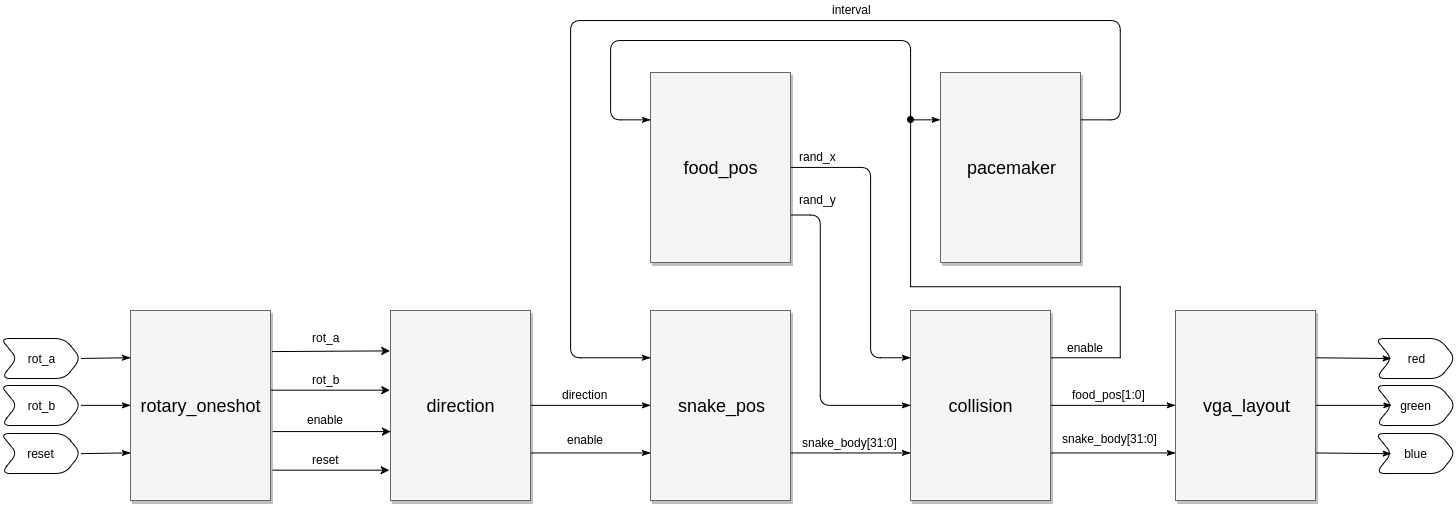
\includegraphics[width=1\textwidth]{top_level_design.png}
            \caption{Block Diagram of the Implementation of the Game}
            \label{fig:schematic}
        \end{center}
    \end{figure}
    \newpage

        \subsection{direction} The \texttt{direction} module is used to control
        the user inputs. The inputs are one-shotted, debounced and fed into the
        internal state machine to determine the direction the user intended.
        This module sets an enable to the \texttt{snake\_pos} module to notify
        a change in direction.

        \begin{figure}[ht]
            \begin{center}
                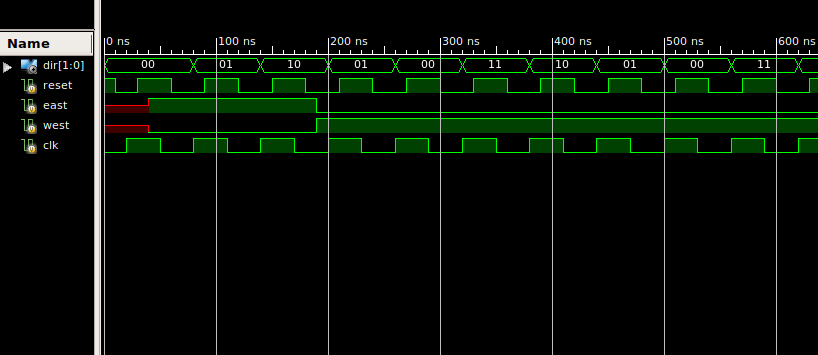
\includegraphics[width=1\textwidth]{direction_wav.png}
                \caption{Waveform of the Testbench of \texttt{direction}}
                \label{fig:direction_wav}
            \end{center}
        \end{figure}

        The sample output demonstrates the \texttt{dir} signal incrementing
        when \texttt{east} is high and decrementing when \texttt{west} is high.

        \subsection{food\_pos} This module generates the \texttt{food\_x} and
        \texttt{food\_y} coordinates of the food when enabled by the
        \texttt{collision} module. The module combinedly utilizes an internal
        counter and a linear feedback shift register to generate the pseudo-
        random coordinates.

        \begin{figure}[ht]
            \begin{center}
                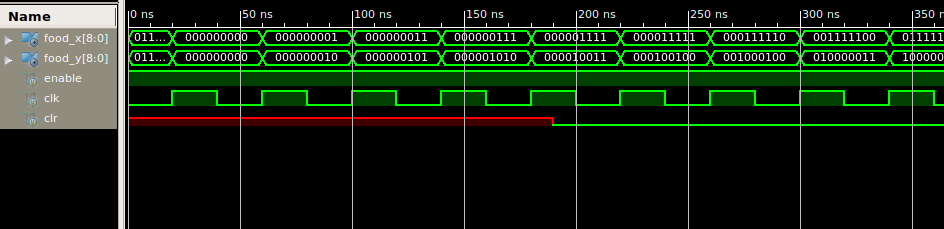
\includegraphics[width=1\textwidth]{food_pos_wav.png}
                \caption{Waveform of the Testbench of \texttt{food\_pos}}
                \label{fig:food_pos_wav}
            \end{center}
        \end{figure}

        The sample output demonstrates the seemingly random coordinates
        generated for \texttt{food\_x} and \texttt{food\_y}.

        \subsection{snake\_pos} The \texttt{snake\_pos} module generates the
        coordinates for the 32 segments of the snake body, including its head.
        The module takes in the 2 bit direction from \texttt{direction} and 2
        enable control signals from \texttt{collision}. The control signals,
        \texttt{grow} and \texttt{dead} are used to indicate the state of the
        snake body. If \texttt{grow} is enabled, the module utilizes
        \texttt{dir} to shift the body segments. If \texttt{dead} is enabled,
        the body segments freeze to indicate end of the game. Its clock is
        timed by \texttt{pacemaker} to control the speed of the moving snake
        body.

        \begin{figure}[ht]
            \begin{center}
                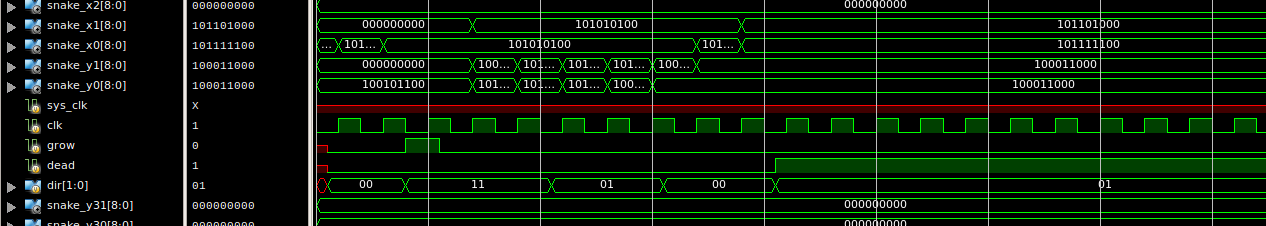
\includegraphics[width=1\textwidth]{snake_pos_wav.png}
                \caption{Waveform of the Testbench of \texttt{snake\_pos}}
                \label{fig:snake_pos_wav}
            \end{center}
        \end{figure}

        The signals were reorganized to highlight the relevant waveforms. The
        sample output demonstrates the movement of the individual body segments
        by utilizing the internal shift register. Only the initial segments
        change due to the snake body's growth being restricted to a length of 2
        in the test bench.

        \subsection{collision} \texttt{collision} accepts the coordinates of
        the food and the snake segments and determines if a collision has been
        detected. If a collision has not been detected, it sends out an enable
        signal to the \texttt{snake\_pos} module. If a collision with the snake
        body, specifically the snake head, with the food is detected, the
        module sends a signal to \texttt{pacemaker} to determine the interval
        at which the snake should move. This module has an internal counter
        that speeds up when the snake head had made 32 collisions with the
        food. If a collision between the snake head and the fence is detected,
        the game is frozen.

        \begin{figure}[ht]
            \begin{center}
                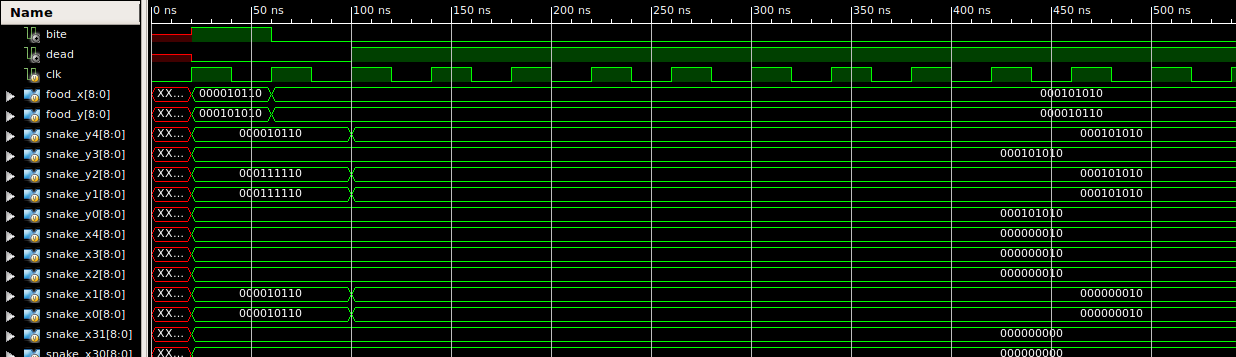
\includegraphics[width=1\textwidth]{collision_wav.png}
                \caption{Waveform of the Testbench of \texttt{collision}}
                \label{fig:collision_wav}
            \end{center}
        \end{figure}

        The signals were reorganized to highlight the relevant waveforms. The
        sample output indicates the conditions to which a collision is
        classified as \texttt{grow} and \texttt{dead}.

        \subsection{vga\_layout} This module draws the fence of the game, and
        the snake and the randomly placed food on the VGA display.

        \subsection{Other Modules} Other minor modules have been utilized for
        the implementation. \texttt{pacemaker} is used to send out control
        signals to the other modules such that they update at reasonable rates.
        The module consists of an internal counter that speeds up the update
        rate once the game has registered over 31 bites of the food.
        \texttt{vga\_sync} is used to synchronize the outputs to the VGA
        display.

\end{document}
